\section{Inicialização}

A inicialização do hipervisor ocorre imediatamente após o controle ser transferido pelo bootloader - U-Boot,
responsável por carregar o binário do hipervisor na memória e transferir a execução para seu ponto de entrada.

O ponto de entrada corresponde a uma função dependente da arquitetura, responsável por realizar a inicialização das
estruturas mais básicas do sistema. Nessa etapa, são configurados os elementos fundamentais de execução da CPU e
do ambiente de hardware, permitindo a transição gradual para camadas superiores do sistema.

A partir dessa função inicial, o controle é transferido sequencialmente para módulos de maior nível de abstração,
até que o sistema alcance o ponto de entrada do escalonador. O fluxo padrão de inicialização segue a seguinte sequência:

\vspace{1cm}

\begin{center}
    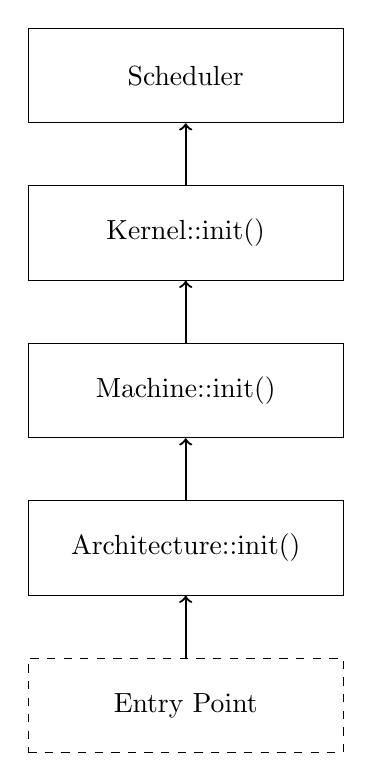
\begin{tikzpicture}
        \node[rectangle, minimum width=4cm, minimum height=1.2cm, draw, align=center, dashed] (A) at (0,0){Entry Point};
        \node[rectangle, minimum width=4cm, minimum height=1.2cm, draw, align=center] (B) at (0,2){Architecture::init()};
        \node[rectangle, minimum width=4cm, minimum height=1.2cm, draw, align=center] (C) at (0,4){Machine::init()};
        \node[rectangle, minimum width=4cm, minimum height=1.2cm, draw, align=center] (D) at (0,6){Kernel::init()};
        \node[rectangle, minimum width=4cm, minimum height=1.2cm, draw, align=center] (E) at (0,8){Scheduler};
        \draw[->, thick] (A) -- (B);
        \draw[->, thick] (B) -- (C);
        \draw[->, thick] (C) -- (D);
        \draw[->, thick] (D) -- (E);
    \end{tikzpicture}
\end{center}

\subsection{Inicialização: RISC-V}

O núcleo da plataforma de virtualização é estabelecido nesta etapa. O papel principal dessa camada de inicialização consiste em instalar os
tratadores de interrupções para a emulação de dispositivos de \gls{mmio} e para o compartilhamento de interrupções entre a máquina hospedeira e os ambientes virtualizados.

A classe responsável por configurar esse vetor de interrupções é a \gls{hic}. O fluxo completo de inicialização é detalhado pelo seguinte diagrama:

\vspace{1cm}

\begin{center}
    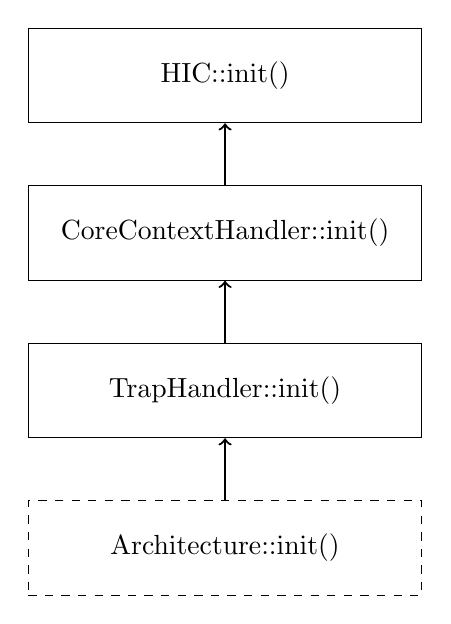
\begin{tikzpicture}
        \node[rectangle, minimum width=5cm, minimum height=1.2cm, draw, align=center, dashed] (A) at (0,2){Architecture::init()};
        \node[rectangle, minimum width=5cm, minimum height=1.2cm, draw, align=center] (B) at (0,4){TrapHandler::init()};
        \node[rectangle, minimum width=5cm, minimum height=1.2cm, draw, align=center] (C) at (0,6){CoreContextHandler::init()};
        \node[rectangle, minimum width=5cm, minimum height=1.2cm, draw, align=center] (D) at (0,8){HIC::init()};
        \draw[->, thick] (A) -- (B);
        \draw[->, thick] (B) -- (C);
        \draw[->, thick] (C) -- (D);
    \end{tikzpicture}
\end{center}


\subsection{Inicialização: Kernel}

Nesta etapa da inicialização do sistema, são executados os rotinas de configuração dos objetos gerais que serão compartilhados
e gerenciados pelo sistema operacional. Esse processo abrange a inicialização de subsistemas críticos, tais como
gerenciamento de memória, estruturas de dados necessárias para o escalonamento de tarefas, etc.

\vspace{1cm}

\begin{center}
    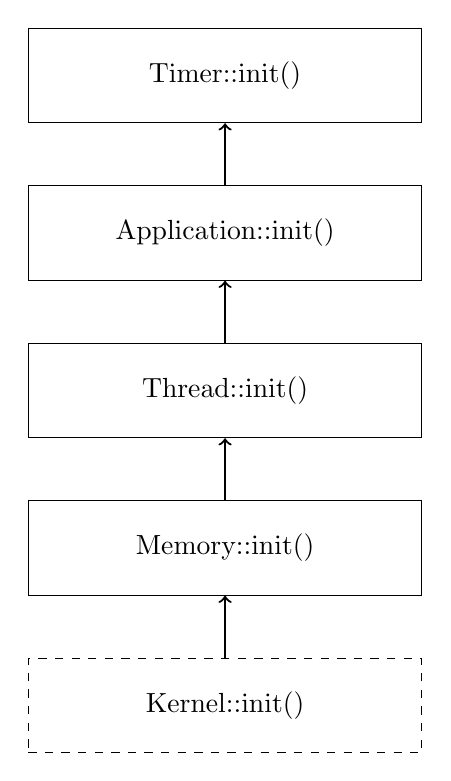
\begin{tikzpicture}
        \node[rectangle, minimum width=5cm, minimum height=1.2cm, draw, align=center, dashed] (A) at (0,2){Kernel::init()};
        \node[rectangle, minimum width=5cm, minimum height=1.2cm, draw, align=center] (B) at (0,4){Memory::init()};
        \node[rectangle, minimum width=5cm, minimum height=1.2cm, draw, align=center] (C) at (0,6){Thread::init()};
        \node[rectangle, minimum width=5cm, minimum height=1.2cm, draw, align=center] (D) at (0,8){Application::init()};
        \node[rectangle, minimum width=5cm, minimum height=1.2cm, draw, align=center] (E) at (0,10){Timer::init()};
        \draw[->, thick] (A) -- (B);
        \draw[->, thick] (B) -- (C);
        \draw[->, thick] (C) -- (D);
        \draw[->, thick] (D) -- (E);
    \end{tikzpicture}
\end{center}


